\documentclass[final]{fhnwreport}       %[mode] = draft or final
                                        %{class} = fhnwreport, article, 
                                        %          report, book, beamer, standalone
%%---Main Packages-----------------------------------------------------------------------
\usepackage[english, ngerman]{babel}	%Mul­tilin­gual sup­port for LaTeX
\usepackage[T1]{fontenc}				%Stan­dard pack­age for se­lect­ing font en­cod­ings
\usepackage[utf8]{inputenc}				%Ac­cept dif­fer­ent in­put en­cod­ings
\usepackage{lmodern}                    %The newer Font-Set
\usepackage{textcomp}					%LaTeX sup­port for the Text Com­pan­ion fonts
\usepackage{graphicx} 					%En­hanced sup­port for graph­ics
\usepackage{float}						%Im­proved in­ter­face for float­ing ob­jects
\usepackage{ifdraft}                    %Let you check if the doc is in draft mode

%%---Useful Packages---------------------------------------------------------------------
\usepackage[pdftex,dvipsnames]{xcolor}  %Driver-in­de­pen­dent color ex­ten­sions for LaTeX
\usepackage{csquotes}                   %Simpler quoting with \enquote{}
\usepackage{siunitx} 					%A com­pre­hen­sive (SI) units pack­age
\usepackage{listings}					%Type­set source code list­ings us­ing LaTeX
\usepackage[bottom]{footmisc}			%A range of foot­note op­tions
\usepackage{footnote}					%Im­prove on LaTeX's foot­note han­dling
\usepackage{verbatim}					%Reim­ple­men­ta­tion of and ex­ten­sions to LaTeX ver­ba­tim
\usepackage[textsize=footnotesize]{todonotes} %Mark­ing things to do in a LaTeX doc­u­ment

%%---Tikz Packages-----------------------------------------------------------------------
\usepackage{standalone}
\usepackage{tikz}
\usepackage{circuitikz}
\usetikzlibrary{arrows}
\usetikzlibrary{calc}
\usetikzlibrary{intersections}

%%---Math Packages-----------------------------------------------------------------------
\usepackage{amsmath}					%AMS math­e­mat­i­cal fa­cil­i­ties for LaTeX
%\usepackage{amssymb}					%Type­set­ting symbols (AMS style)
%\usepackage{array}						%Ex­tend­ing the ar­ray and tab­u­lar en­vi­ron­ments
%\usepackage{amsthm}					%Type­set­ting the­o­rems (AMS style)

%%---Table Packages----------------------------------------------------------------------
\usepackage{tabularx}					%Tab­u­lars with ad­justable-width columns
%\usepackage{longtable}
\usepackage{multirow}					%Create tab­u­lar cells span­ning mul­ti­ple rows
\usepackage{multicol}					%In­ter­mix sin­gle and mul­ti­ple columns

%%---PDF / Figure Packages---------------------------------------------------------------
\usepackage{pdfpages}					%In­clude PDF doc­u­ments in LaTeX
\usepackage{pdflscape}					%Make land­scape pages dis­play as land­scape
\usepackage{subfig}					    %Fig­ures di­vided into sub­fig­ures

%%---Other Packages----------------------------------------------------------------------
%\usepackage{xargs}                     %De­fine com­mands with many op­tional ar­gu­ments

%%---Bibliography------------------------------------------------------------------------
\usepackage[style=ieee,urldate=comp,backend=biber]{biblatex}
\addbibresource{literature/bibliography.bib}

%%---Main Settings-----------------------------------------------------------------------
\graphicspath{{./graphics/}}			%Defines the graphicspath
%\geometry{twoside=false}				    %twoside=false disables the "bookstyle"
\setlength{\marginparwidth}{2cm}
\overfullrule=5em						%Creates a black rule if text goes over the margins => debugging


%%---User Definitions--------------------------------------------------------------------
%%Tabel-Definitions: (requires \usepackage{tabularx})
\newcolumntype{L}[1]{>{\raggedright\arraybackslash}p{#1}}    %column-width and alignment
\newcolumntype{C}[1]{>{\centering\arraybackslash}p{#1}}
\newcolumntype{R}[1]{>{\raggedleft\arraybackslash}p{#1}}

%%---Optional Package Settings-----------------------------------------------------------
%Listings-Settings: (requires \usepackage{listings}) => Example with Matlab Code
\lstset{language=Matlab,%
    basicstyle=\footnotesize\ttfamily,
    breaklines=false,%
    morekeywords={switch, case, otherwise},
    keywordstyle=\color{Blue},%
    tabsize=2,
    %morekeywords=[2]{1}, keywordstyle=[2]{\color{black}},
    identifierstyle=\color{Black},%
    stringstyle=\color{Purple},
    commentstyle=\color{Green},%
    showstringspaces=false,%without this there will be a symbol in the places where there is a space
    numbers=left,%
    numberstyle={\tiny \color{black}},% size of the numbers
    numbersep=9pt, % this defines how far the numbers are from the text
    %emph=[1]{word1, word2,...},emphstyle=[1]\color{red}
}										                %loads all packages, definitions and settings												
\title{Balun}          %Project Title
\author{Bericht hf1}          %Document Type => Technical Report, ...
\date{Windisch, \today}             %Place and Date

\begin{document}

%%---TITLEPAGE---------------------------------------------------------------------------
\selectlanguage{ngerman}                %ngerman or english
\maketitle

\vspace*{-1cm}						    %compensates the space after the date line.
\vfill
\begin{figure}[H]
\centering

\includegraphics[width=\linewidth]{titelbild.pdf}
\end{figure}
\vfill

{
\renewcommand\arraystretch{2}
\begin{center}
\begin{tabular}{>{\bf}p{4cm} l}
Hochschule                 &    Hochschule für Technik - FHNW\\
Studiengang                &    Elektro- und Informationstechnik\\
Autor   		           & 	Adrian Annaheim und Alexander Stutz\\
Betreuer                   &    Peter Niklaus\\
Version                    &    1.0 %Normally not used!
\end{tabular}
\end{center}
}

\clearpage
			
%%---ABSTRACT----------------------------------------------------------------------------
\selectlanguage{ngerman}				%ngerman or english
\thispagestyle{empty}
\begin{abstract}
Das Abstract ist eine Art Zusammenfassung des ganzen Dokuments. Es gibt einen Einblick in die Aufgabenstellung, wie diese umgesetzt wurde und welches Ergebnis erreicht wurde. Aus diesem Grund wird das Abstract immer ganz am Schluss der Arbeit verfasst. Es besteht aus einem zusammengehörenden Absatz und umfasst ungefähr 10 bis 20 Zeilen.
Formeln, Referenzen oder andere Unterbrechungen haben im Text nichts zu suchen.
Direkt unter dem Abstract folgt eine Liste von drei bis vier Stichworten/Keywords. Diese werden in alphabetischer Reihenfolge aufgelistet und beschreiben das Themengebiet der Arbeit.

\vspace{2ex}
\textbf{Keywords: Anleitung, LaTeX, Thesis, Vorlage}
\end{abstract}	


\vfill

\begin{center}
\color{green!50!black!100}\bf
Bitte schicken Sie jeglichen Feedback auch an \texttt{hanspeter.schmid@fhnw.ch}\\
Er wird dieses Template langfristig unterhalten.
\end{center}

\vfill
\null

%%---TABLE OF CONTENTS-------------------------------------------------------------------
\pagenumbering{Roman}		
\selectlanguage{ngerman}				%ngerman or english
\tableofcontents
\clearpage

%%---TEXT--------------------------------------------------------------------------------
\pagenumbering{arabic}
\section{Problemstellung}
In der HF-Technik kommt es sehr oft zur Situation, in welcher zwei Komponenten miteinander verbunden werden. Dieses auf den ersten Blick simple Vorhaben, kann einige Probleme bereiten. Haben die Komponenten unterschiedliche Impedanzen, spricht man von Fehlanpassung und es treten unerwünschte Reflexionen in der Leitung auf. Diese führen zu Verlusten und Verzerrungen des Signals. In diesem Bericht wird nun folgende Ausgangslage genauer betrachtet:
\begin{figure}[h]
	\centering
	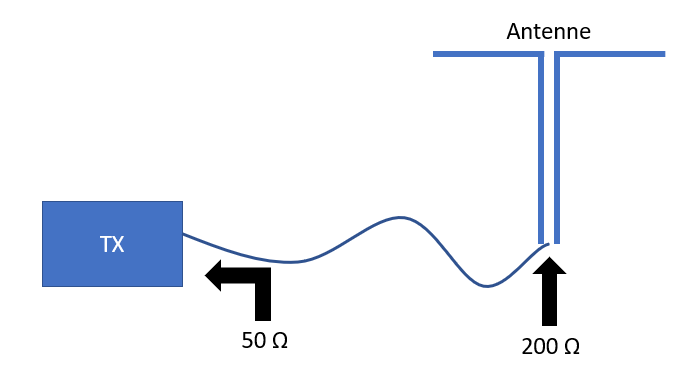
\includegraphics[width=0.6\linewidth]{ausgangslage.png}
	\caption{Ausgangslage Quelle an Antenne}\label{fig:ausgangslage}
\end{figure}

Eine 50$\Omega$-Quelle wird an eine 200$\Omega$-Dipol-Antenne angeschlossen. Schliesst man die Antenne direkt an die Quelle wie in Abbildung \ref{fig:ausgangslage}, kommt es zur Fehlanpassung und den erwähnten Effekten. Die Impedanzanpassung ist jedoch nicht die einzige Herausforderung dieser Konstellation.
\newline
Weil nur die wenigsten Dipol-Antennen symmetrisch sind, fliessen Gleichtakt-Ausgleichsströme auf dem Aussenmantel der Leitung. Dadurch strahlt die Leitung ab und empfängt Störungen. Um diesen Sachverhalt genauer zu verstehen, betrachten wir zuerst eine ideale Dipol-Antenne.

\begin{figure}[H]
	\centering
	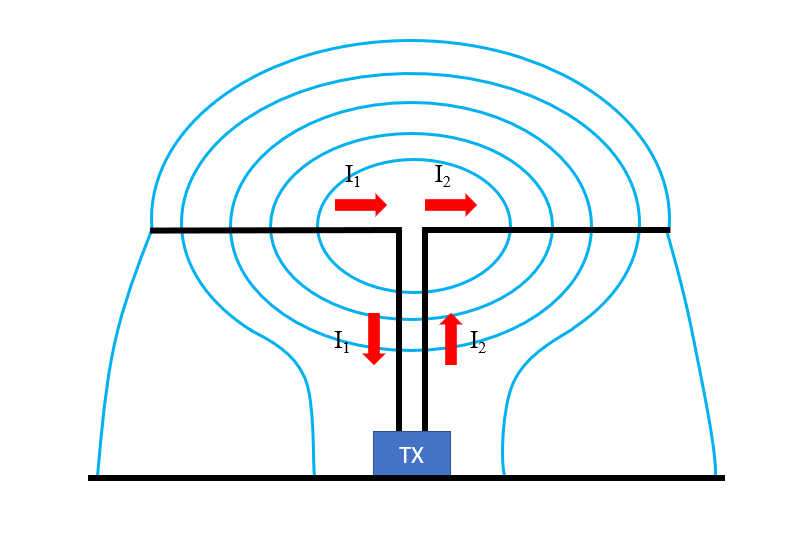
\includegraphics[width=0.8\linewidth]{idealer_dipol.png}
	\caption{Ströme und Felder bei einer idealen Dipol-Antenne}\label{fig:idealer_dipol}
\end{figure}

Sind beide Dipoläste exakt symmetrisch, sind die Impedanzen der einzelnen Äste gleich. Damit gilt für die Ströme $I_{1}=-I_{2}$. Sind die Ströme im Kabel Betragsgleich und entgegengesetzt, heben sich die Felder auf und die Leitung strahlt nicht ab.



\section{Grundlagen}

Sowohl das Problem der störenden Mantelwellen als auch die Fehlanpassung der Antenne an das Koaxialkabel lässt sich mittels eines sogenannten Baluns lösen. Ein solcher kann auf verschiedene Wege realisiert werden. Grundsätzlich unterscheidet man dabei zwischen Strom- und Spannungsbalun. Natürlich gibt es auch Hybride aus beiden Typen. 

\subsection{Spannungsbalun}
Ein Spannungsbalun transformiert eine unsymmetrische in eine symmetrische Spannung. Dies kann zum Beispiel durch einen Transformator, so wie in Abbildung \ref{fig:Spannungsbalun} gezeigt, erreicht werden. 
Falls die Antenne ideal symmetrisch ist, kann damit das nicht symmetrische Koaxialkabel an die Antenne angepasst werden. Ideal symmetrisch bedeutet, dass die beiden Dipole eine identische kapazitive und induktive Kopplung zur Erde haben. 
Durch das Windungszahlverhältnis kann eine beliebige Impedanzanpassung realisiert werden. 
Da die gesamte Energie, welche den Balun passiert, als Magnetfeld durch den Kern fliesst, muss dieser eine hohe Güte haben.
\begin{figure}[H]
	\centering
	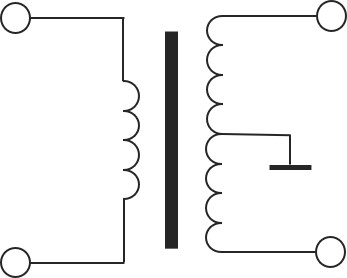
\includegraphics[width=0.3\linewidth]{Spannungsbalung.jpg}
	\caption{Einfaches Beispiel für einen Spannungsbalun}\label{fig:Spannungsbalun}
\end{figure}

\subsection{Strombalun}
\label{sec:strombalun}
Ein Strombalun zwingt der Leitung einen symmetrischen Strom auf. Dabei werden die störenden Mantelwellen idealerweise unterdrückt. Ein einfaches Beispiel für einen Strombalun ist in Abbildung \ref{fig:Strombalun} ersichtlich. Da sich bei dieser Schaltung die beiden Magnetfelder für das gewünschte Gegentaktsignal aufheben, fliesst nur die Energie des störenden Signals als Magnetfeld durch den Kern. Dieser darf deshalb eine niedrigere Güte haben. Das kann sogar gewünscht sein, da dadurch das störenden Gleichtaktsignal in Wärme umgewandelt wird und eine tiefe Güte ausserdem einen breitbandigen Betrieb ermöglicht. Aufgrund der Eigenschaft dass der Strombalun Mantelwellen zumindest dämpft, kann er auch bei nicht idealen Dipolantennen verwendet werden. Eine Impedanzanpassung ist bei der klassischen Schaltung in der Abbildung \ref{fig:Strombalun} nicht möglich.
\begin{figure}[H]
	\centering
	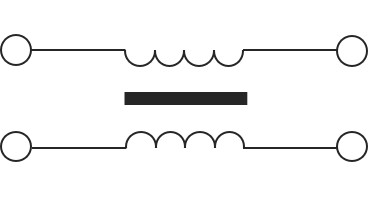
\includegraphics[width=0.3\linewidth]{Strombalun.jpg}
	\caption{Einfaches Beispiel für einen Strombalun}\label{fig:Strombalun}
\end{figure}

\newpage
\subsubsection{Guanella-Balun}
Der Guanella-Balun ist ein Spezialfall des Strombaluns, bei welchem durch Zusammenschalten von mehreren klassischen Stufen eine Impedanzanpassung für bestimmte Verhältnisse erreicht werden kann. In Abbildung \ref{fig:Guanella} ist ein Beispiel mit zwei Stufen ersichtlich. Unter der Annahme, dass die beiden Strombalune ideal funktionieren, fliessen die mit orangen Pfeilen eingezeichnete Ströme. Auf der linken Seite addieren sich je zwei Strompfade zusammen, wodurch der Strom, welcher von links in den Balun fliesst, doppelt so gross ist, wie der Strom auf der auf rechten Seite. Da die Schaltung idealerweise keine Verlustbehafteten Komponenten enthält muss die Eingangsleistung gleich gross wie die Ausgangsleistung sein. Daraus folgt, dass die Spannung auf der rechten Seite doppelt so gross wie links sein muss. Das Impedanzverhältniss berechnet sich wie folgt: \cite{balun_work} \cite{sevik} 
\begin{equation}
\frac{Z_2}{Z_1}=\frac{U_2/I_2}{U_1/I_1}=\frac{2\cdot U_1/I_2}{U_1/(2\cdot I_2)}=4:1
\label{equ:Guanella_1}
\end{equation}

Durch Hinzufügen von weiteren Stufen lassen sich folgende Verhältnisse realisieren:
\begin{equation}
	\frac{Z_{out}}{Z_{in}}=n^{2}:1 \hspace{1cm} n\in\mathrm{N}
\end{equation}
\begin{figure}[H]
	\centering
	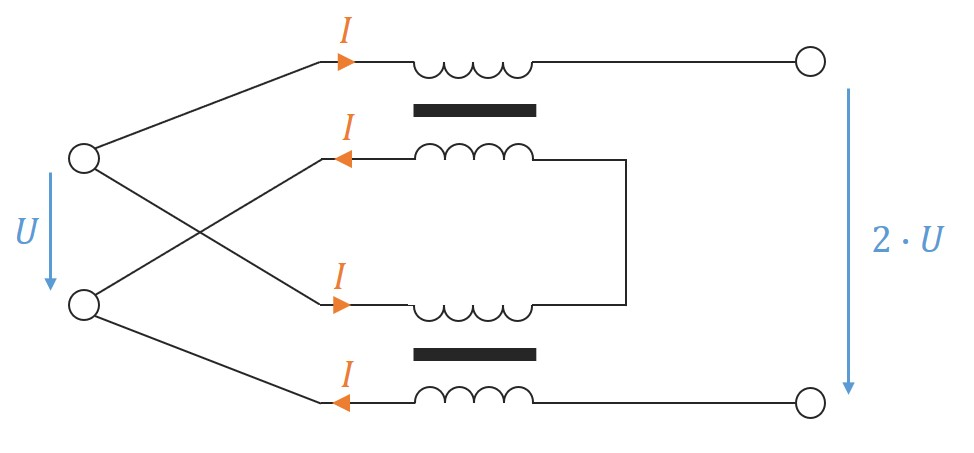
\includegraphics[width=1\linewidth]{Guanella.jpg}
	\caption{Ein Guanella-Balun mit zwei Stufen.}\label{fig:Guanella}
\end{figure}
\section{Dimensionierung des Baluns}

\section{Validierung}
Damit das Verhalten des gebauten Baluns getestet werden kann, werden die beiden Aufgaben, die Impedanzanpassung und das Erzwingen symmetrischer Ströme, unabhängig voneinander überprüft.
\subsection{Impedanzanpassung}
Um die Impedanzanpassung zu verifizieren, wurde am Ausgang des Baluns eine Last von \SI{200}{\Omega} angeschlossen. Da es sich um einen Guanella-Balun mit einem Übersetzungsverhältnis von 1:4 handelt, muss man am Eingang nun eine Impedanz von \SI{50}{\Omega} sehen. Dies wurde mit zwei Messungen überprüft.

\paragraph{Impedanzmessung}
Mit folgender Messanordnung wurde die Impedanz des Baluns direkt gemessen. Das Messresultat ist in Abbildung \ref{fig:Eingangsimpedanz2} ersichtlich.
\begin{figure}[H]
	\centering
	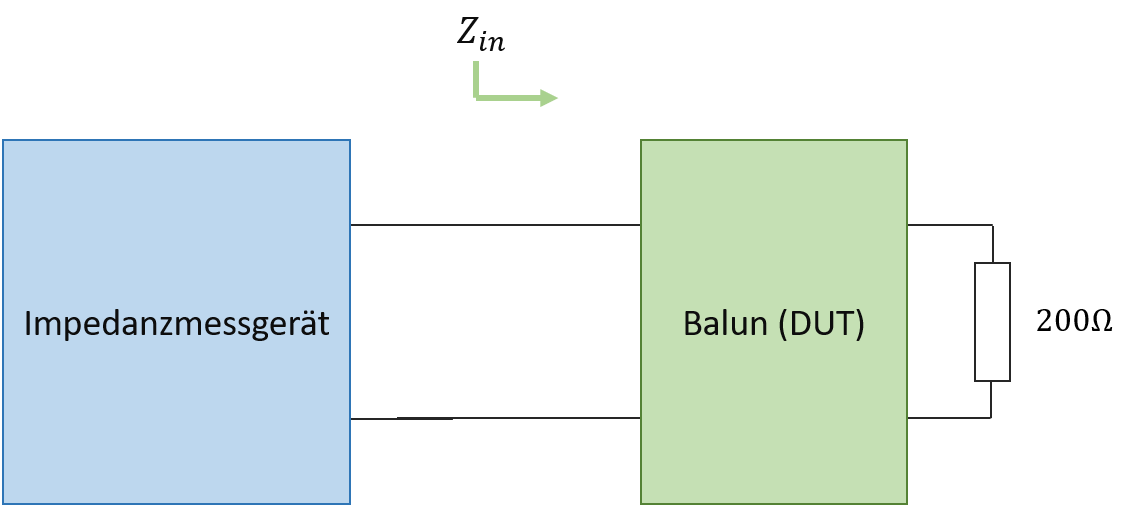
\includegraphics[width=0.6\linewidth]{Messaufbau_Eingangsimpedanz_2.png}
	\caption{Eingangsimpedanz in logarithmischer Darstellung}\label{fig:mess_eingangsimpedanz2}
\end{figure}

\begin{figure}[H]
	\centering
	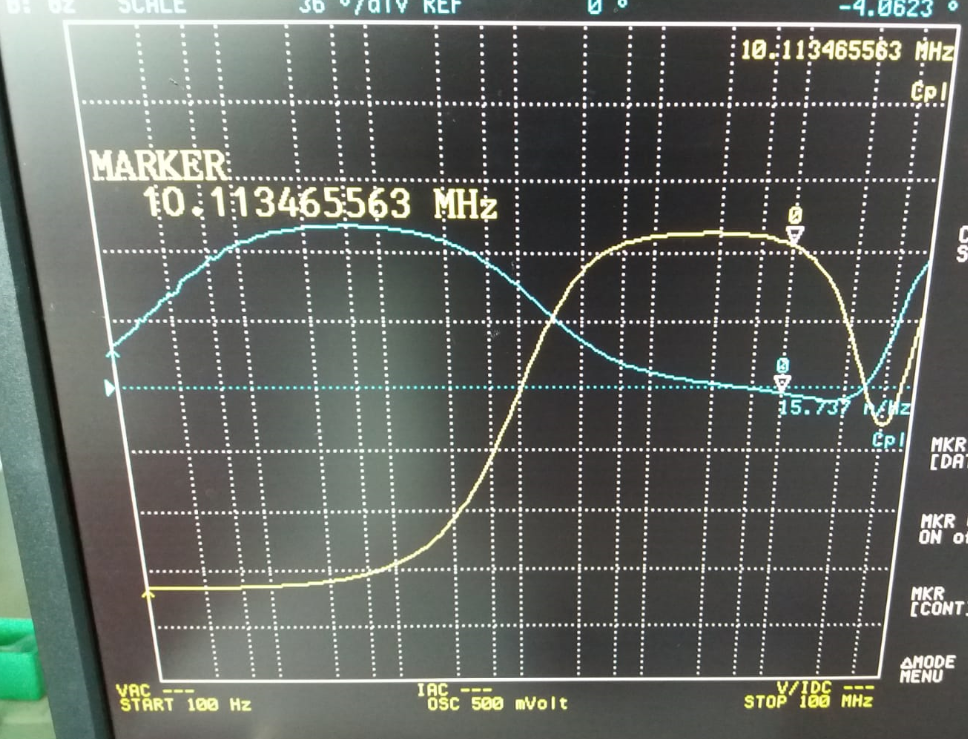
\includegraphics[width=0.6\linewidth]{Eingangsimpedanz2.PNG}
	\caption{Eingangsimpedanz in logarithmischer Darstellung}\label{fig:Eingangsimpedanz2}
\end{figure}
Liegt die gemessene Impedanz in der Nähe von \SI{50}{\Omega} funktioniert die Impedanzanpassung. Wie zu erkennen ist, ist dies im Bereich zwischen \SI{200}{kHz} und \SI{10}{MHz} der Fall. Bei tiefen Frequenzen funktioniert die Impedanzanpassung nicht, weil die Wirkung der einzelnen Wicklungen noch zu schwach ist. Bei höheren Frequenzen beginnt die Wicklungskapazität zu wirken.

\paragraph{Reflexionsmessung}
Auch hier wird überprüft, ob die Eingangsimpedanz \SI{50}{\Omega} beträgt. Dazu wird der Balun in ein \SI{50}{\Omega}-Netzwerk integriert und auf Reflexionen untersucht. Die dafür verwendete Messschaltung ist in Abbildung \ref{fig:mess_eingangsimpedanz} gezeigt.
\begin{figure}[H]
	\centering
	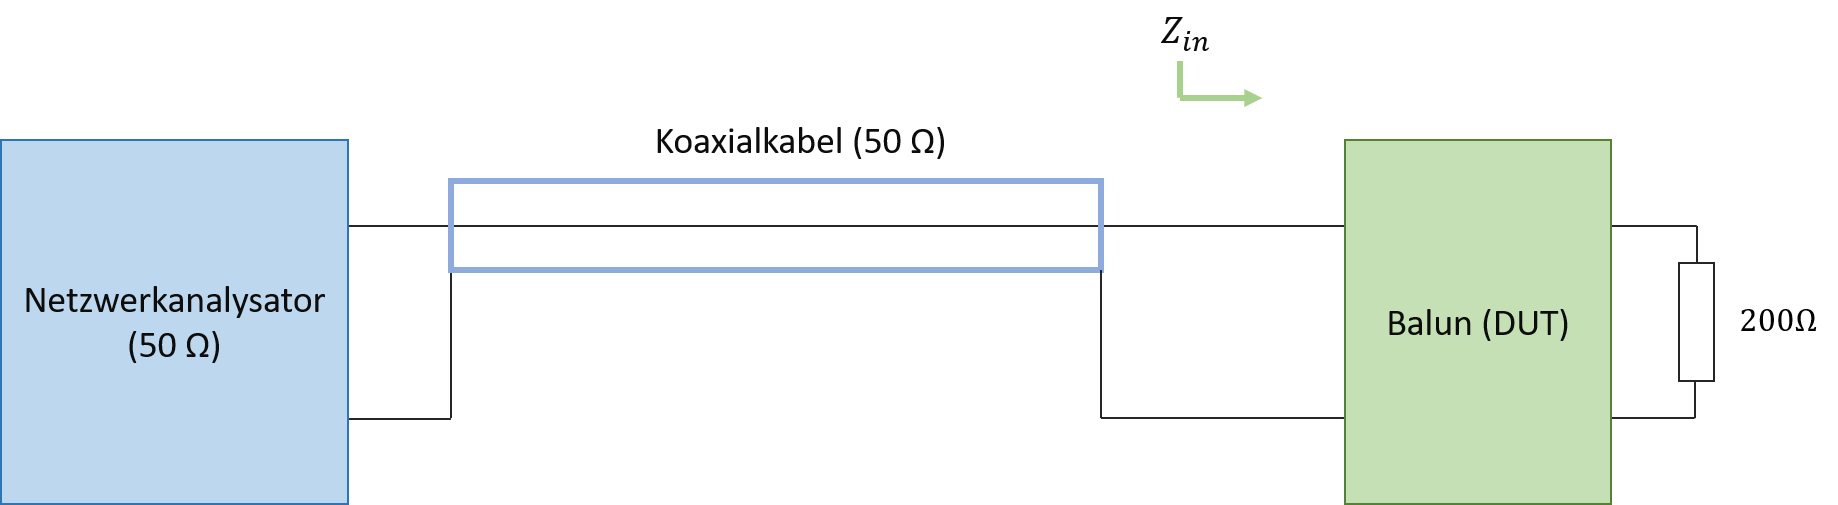
\includegraphics[width=0.7\linewidth]{Messaufbau_Eingangsimpedanz.png}
	\caption{Eingangsimpedanz in logarithmischer Darstellung}\label{fig:mess_eingangsimpedanz}
\end{figure}

\begin{figure}[H]
	\centering
	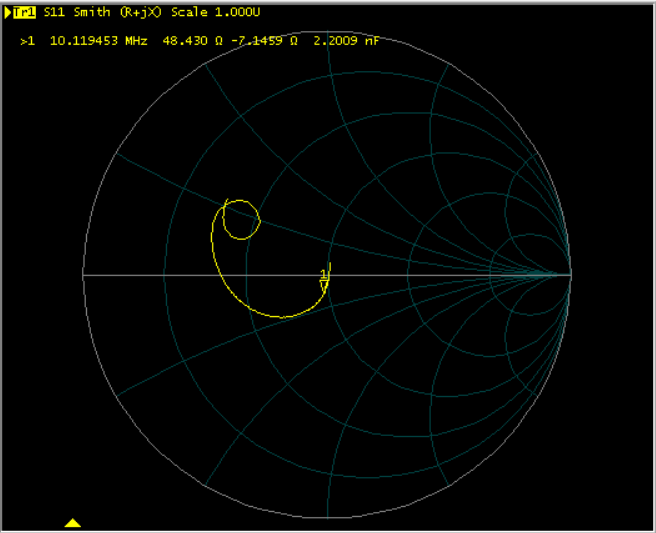
\includegraphics[width=0.7\linewidth]{Eingangsimpedanz.PNG}
	\caption{Eingangsimpedanz dargestellt in der Smith-Chart}\label{fig:Eingangsimpedanz}
\end{figure}

In der Abbildung \ref{fig:Eingangsimpedanz} ist die gemessene Reflexion in der Smith-Chart dargestellt. Wie erwartet, deckt sich das Ergebnis mit der vorherigen Impedanzmessung.
\newpage
\subsection{Symmetrische Ströme}

Um die zweite Aufgabe des Baluns, das Erzwingen symmetrischer Ströme, zu verifizieren, haben wir die im folgenden dargestellte Messung durchgeführt.
\begin{figure}[H]
	\centering
	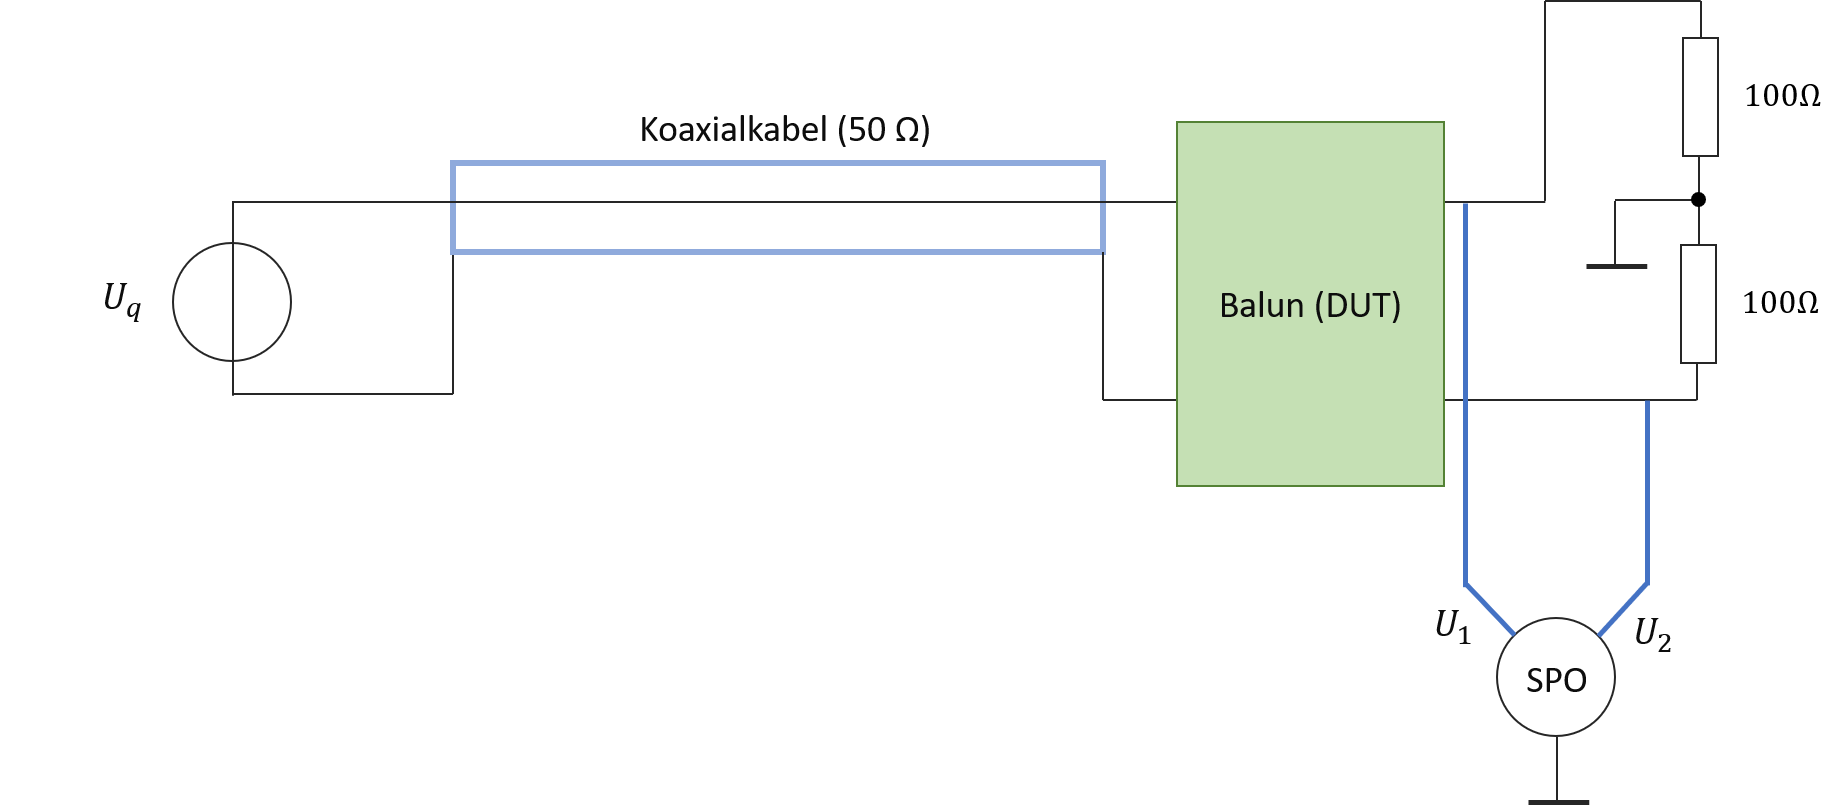
\includegraphics[width=0.8\linewidth]{Messaufbau_Symetrie_1.png}
	\caption{Eingangsimpedanz dargestellt in der Smith-Chart}\label{fig:mess_sym}
\end{figure}
Die beiden Widerstände am Ausgang bilden eine symmetrische Last. Ohne Balun würde die gesamte Spannung über einem der Widerstände abfallen. Bei korrekter Funktion des Baluns liegt an beiden Widerständen die selbe Spannung mit einer Phasenverschiebung von \SI{180}{^\circ} an.\\
In folgender Abbildung ist das Verhältnis der beiden Amplitudenbeträge dargestellt. Man erkennt, dass der Balun zwischen \SI{5}{MHz} und \SI{80}{MHz} symmetrische Stromamplituden erzeugt. \cite{balun_work}
\cite{balun_meas}
\begin{figure}[H]
	\centering
	\includegraphics[width=0.75\linewidth]{Betrag_Sym.PNG}
	\caption{Eingangsimpedanz dargestellt in der Smith-Chart}\label{fig:Betrag_sym}
\end{figure}
Nun wird überprüft, ob die Phasenverschiebung \SI{180}{^\circ} beträgt. Wie man in Abbildung \ref{fig:Phase_sym} erkennen kann, ist dies praktisch über dem ganzen Messbereich der Fall.
\begin{figure}[H]
	\centering
	\includegraphics[width=0.8\linewidth]{Phase_Sym.PNG}
	\caption{Eingangsimpedanz dargestellt in der Smith-Chart}\label{fig:Phase_sym}
\end{figure}
\section{Erkenntnisse}
Die Validierung hat folgendes aufgezeigt: Bei der gewählten Arbeitsfrequenz von \SI{20}{MHz} erzwingt der Guanella-Balun wie gewünscht symmetrische Ströme. Die Impedanzanpassung funktioniert jedoch nur bis zu einer Frequenz von ca. \SI{10}{MHz}. Diese obere Grenzfrequenz wird durch das Verhältnis von Wicklungskapazität zu Induktivität bestimmt, und kann deshalb wie folgt erhöht werden:
\begin{itemize}
	\item Abstand zwischen der Wicklungen erhöhen
	\item Anzahl der Wicklungen erhöhen
\end{itemize}

Damit solche Änderungen keine Einflüsse auf die Resonanzfrequenz des Baluns haben, muss ein anderer Parameter, wie zum Beispiel der Kern, entsprechend verändert werden.
\vspace{1cm}
Möchte man den realisierten Balun ohne Änderungen verwenden, muss eine andere Arbeitsfrequenz gewählt werden. In Frage kommen die Frequenzbereiche, bei welchen sowohl die Impedanzanpassung als auch die Symmetriebedingung erfüllt ist. Dies ist zwischen ungefähr zwischen \SI{5}{MHz} und \SI{10}{MHz} der Fall. 
\vspace{1cm}


\section{Schlusswort}
Im Verlaufe dieser Arbeit hat sich gezeigt, dass bei der Realisierung eines Baluns relativ viel mit Abschätzen und Nachjustieren gearbeitet werden muss. Dies gilt besonders bei der Verwendung von gekoppelten Spulen und der Herstellung von Hand.
Da es keine allgemein gültige Anleitung zur Dimensionierung eines Baluns gibt, gestattet sich die Definition eines Models als heikel.

%%---BIBLIOGRAPHY------------------------------------------------------------------------
{\sloppypar
\printbibliography[heading=bibintoc]
\label{sec:lit}
\selectlanguage{english}				%ngerman or english
\printbibliography[heading=bibintoc]
}

%%---APPENDIX----------------------------------------------------------------------------
\begin{appendix} %Anhang




\end{appendix}


%%---NOTES for DEBUG---------------------------------------------------------------------
\ifdraft{%Do this only if mode=draft
%%requires \usepackage{todonotes})
\newpage
\listoftodos[\section{Todo-Notes}]
\clearpage
}
{%Do this only if mode=final
}
\end{document}
